\section{Model1D  Class Reference}
\label{classModel1D}\index{Model1D@{Model1D}}
A simple one-dimensional model for dynamics studies. 


{\tt \#include $<$modelmisc.h$>$}

Inheritance diagram for Model1D::\begin{figure}[H]
\begin{center}
\leavevmode
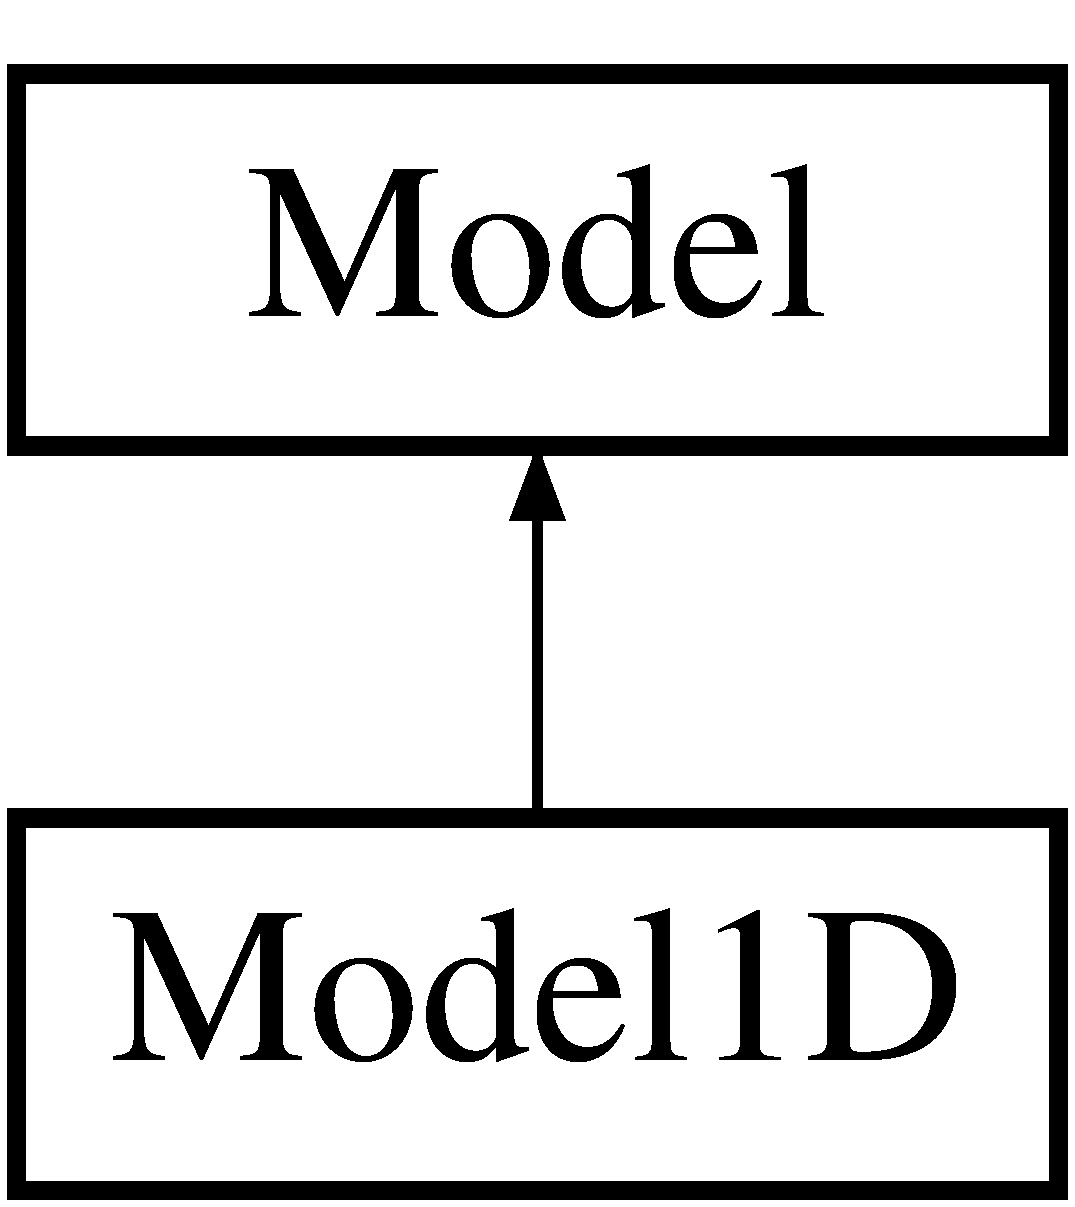
\includegraphics[height=2cm]{classModel1D}
\end{center}
\end{figure}
\subsection*{Public Methods}
\begin{CompactItemize}
\item 
{\bf Model1D} (string path)
\item 
virtual {\bf $\sim$Model1D} ()
\item 
virtual {\bf MSLVector} {\bf State\-To\-Configuration} (const {\bf MSLVector} \&{\bf x})
\begin{CompactList}\small\item\em A method that converts a {\bf Model} {\rm (p.\,\pageref{classModel})} state in to a {\bf Geom} {\rm (p.\,\pageref{classGeom})} configuration.\item\end{CompactList}\item 
virtual {\bf MSLVector} {\bf Integrate} (const {\bf MSLVector} \&{\bf x}, const {\bf MSLVector} \&u, const double \&h)
\begin{CompactList}\small\item\em Perform integration from state x, using input u, over time step h.\item\end{CompactList}\item 
virtual {\bf MSLVector} {\bf State\-Transition\-Equation} (const {\bf MSLVector} \&{\bf x}, const {\bf MSLVector} \&u)
\begin{CompactList}\small\item\em The state transition equation, or equations of motion, xdot=f(x,u).\item\end{CompactList}\item 
virtual double {\bf Metric} (const {\bf MSLVector} \&x1, const {\bf MSLVector} \&x2)
\begin{CompactList}\small\item\em A distance metric, which is Euclidean in the base class.\item\end{CompactList}\end{CompactItemize}
\subsection*{Public Attributes}
\begin{CompactItemize}
\item 
double {\bf Force}
\end{CompactItemize}


\subsection{Detailed Description}
A simple one-dimensional model for dynamics studies.



\subsection{Constructor \& Destructor Documentation}
\index{Model1D@{Model1D}!Model1D@{Model1D}}
\index{Model1D@{Model1D}!Model1D@{Model1D}}
\subsubsection{\setlength{\rightskip}{0pt plus 5cm}Model1D::Model1D (string {\em path})}\label{classModel1D_a0}


\index{Model1D@{Model1D}!~Model1D@{$\sim$Model1D}}
\index{~Model1D@{$\sim$Model1D}!Model1D@{Model1D}}
\subsubsection{\setlength{\rightskip}{0pt plus 5cm}virtual Model1D::$\sim$Model1D ()\hspace{0.3cm}{\tt  [inline, virtual]}}\label{classModel1D_a1}




\subsection{Member Function Documentation}
\index{Model1D@{Model1D}!Integrate@{Integrate}}
\index{Integrate@{Integrate}!Model1D@{Model1D}}
\subsubsection{\setlength{\rightskip}{0pt plus 5cm}{\bf MSLVector} Model1D::Integrate (const {\bf MSLVector} \& {\em x}, const {\bf MSLVector} \& {\em u}, const double \& {\em h})\hspace{0.3cm}{\tt  [virtual]}}\label{classModel1D_a3}


Perform integration from state x, using input u, over time step h.



Implements {\bf Model} {\rm (p.\,\pageref{classModel_a5})}.\index{Model1D@{Model1D}!Metric@{Metric}}
\index{Metric@{Metric}!Model1D@{Model1D}}
\subsubsection{\setlength{\rightskip}{0pt plus 5cm}double Model1D::Metric (const {\bf MSLVector} \& {\em x1}, const {\bf MSLVector} \& {\em x2})\hspace{0.3cm}{\tt  [virtual]}}\label{classModel1D_a5}


A distance metric, which is Euclidean in the base class.



Reimplemented from {\bf Model} {\rm (p.\,\pageref{classModel_a9})}.\index{Model1D@{Model1D}!StateToConfiguration@{StateToConfiguration}}
\index{StateToConfiguration@{StateToConfiguration}!Model1D@{Model1D}}
\subsubsection{\setlength{\rightskip}{0pt plus 5cm}{\bf MSLVector} Model1D::State\-To\-Configuration (const {\bf MSLVector} \& {\em x})\hspace{0.3cm}{\tt  [virtual]}}\label{classModel1D_a2}


A method that converts a {\bf Model} {\rm (p.\,\pageref{classModel})} state in to a {\bf Geom} {\rm (p.\,\pageref{classGeom})} configuration.



Reimplemented from {\bf Model} {\rm (p.\,\pageref{classModel_a8})}.\index{Model1D@{Model1D}!StateTransitionEquation@{StateTransitionEquation}}
\index{StateTransitionEquation@{StateTransitionEquation}!Model1D@{Model1D}}
\subsubsection{\setlength{\rightskip}{0pt plus 5cm}{\bf MSLVector} Model1D::State\-Transition\-Equation (const {\bf MSLVector} \& {\em x}, const {\bf MSLVector} \& {\em u})\hspace{0.3cm}{\tt  [virtual]}}\label{classModel1D_a4}


The state transition equation, or equations of motion, xdot=f(x,u).



Implements {\bf Model} {\rm (p.\,\pageref{classModel_a3})}.

\subsection{Member Data Documentation}
\index{Model1D@{Model1D}!Force@{Force}}
\index{Force@{Force}!Model1D@{Model1D}}
\subsubsection{\setlength{\rightskip}{0pt plus 5cm}double Model1D::Force}\label{classModel1D_m0}




The documentation for this class was generated from the following files:\begin{CompactItemize}
\item 
{\bf modelmisc.h}\item 
{\bf modelmisc.C}\end{CompactItemize}
